\documentclass[12pt, A4]{report}

% Packages
	% Basics
		\usepackage{amsmath}
		\usepackage{bm}
		\usepackage{cellspace}
		\usepackage{cite}
		\usepackage{csquotes}
		\usepackage{fixltx2e}
		\usepackage[hang,flushmargin]{footmisc}
		\usepackage{float}
		\usepackage[margin=0.75in]{geometry}
		\usepackage{graphicx}
		\usepackage{hyperref}
		\usepackage[utf8]{inputenc}
		\usepackage{subcaption}
	% Diagrams
		\usepackage{pgfplots}
		\usepackage{tikz}
			\usepackage{circuitikz} % Circuits
			\usepackage{tikz-3dplot} % 3D
			\usetikzlibrary{arrows.meta, angles, calc, quotes}
	% Notation
		\usepackage{amssymb} % Miscellaneous
		\usepackage{chemformula}
		\usepackage{esint} % Integrals
		\usepackage{physics} % Differentials/Vectors
% Macros
	% Notation
		% Constants
			\DeclareMathOperator{\en}{e}
		% Distributions
			\newcommand{\Exp}{\mathbb{E}}
			\newcommand{\ndist}{\mathcal{N}}
			\DeclareMathOperator{\vari}{var}
		% Functions
			\DeclareMathOperator{\erfc}{erfc}
		% Sets
			\newcommand{\R}{\mathbb{R}}
		% Other
			\DeclareMathOperator{\avg}{avg}
			\renewcommand{\th}{\text{th}}
	% Utilities
		\newcommand{\callout}[2]{\begin{center}\fbox{\begin{minipage}{#1cm}#2\end{minipage}}\end{center}}
		\newcommand{\comment}[1]{}
		\newcommand{\subsectionb}[1]{\subsection*{#1}\addcontentsline{toc}{subsection}{#1}}
		\newcommand{\subsubsectionb}[1]{\subsubsection*{#1}\addcontentsline{toc}{subsubsection}{#1}}

% Configuration
	\title{Use of Stochastic Calculus to Predict Stock Market Trends}
	\author{Arnav Patri and Shashank Chidige}
	\date{}
	\hypersetup{
	    colorlinks,
	    citecolor=cyan,
	    filecolor=cyan,
	    linkcolor=cyan,
	    urlcolor=cyan
	}
	\cellspacetoplimit10pt
	\cellspacebottomlimit10pt


\begin{document}
	\maketitle
	\noindent
	The aim of this project is to use differential equations to determine a method by which the behavior of stock prices can be modeled to gain financial insight. There are simply too many variables that have an impact on a stock's price, though, not all of which can be individually accounted for. The problem of optimizing buy and sell times of stocks is affected by the multitude of internal and external forces that affect the stock's price. In business, political, economic, social, and technological changes in the business environment can impact a stock's price. Rather than attempting to account for every individual variable, the aggregate result can be modeled stochastically. \\
	Despite its complexity, an understanding of both statistics and differential equations being required, stochastic calculus enables traders to make more informed predictions regarding stock prices. Many firms already employ stochastic models for this reason. They stand to gain financially by increasing the accuracy of their prediction. In fact, many trading services directly incorporate stochastic models unbeknownst to those using them. \\
	The model being employed is
		\[\dv{S_t}{t} = \mu S_t + \sigma S_t\dv{W_t}{t}\]
		where \(t\) is time (the independent variable), \(S_t\) is the stock price (as a function of time), \(\mu\) is the (constant) expected return on the stock, \(\sigma\) is the (constant) volatility (standard deviation), and \(W_t\) is a standard Wiener process, with mean 0 and variance 1, as adapted from \cite{Stochastic}. \\
		The Wiener process is stochastic, meaning that its value changes over time randomly. As such, only the distribution of possible values is known at any given point in time. This distribution is defined by the mean and variance, in this case 0 and 1 respectively. The Wiener process is a series of randomly distributed normal variables with variances that increase over time, reflecting the increasing uncertainty in making predictions further into the future. \\
		The change in the Wiener process can be found as
		\[\Delta W = \varepsilon\sqrt{\Delta t}\]
		where \(\varepsilon \sim \ndist(0, 1)\) (\(\varepsilon\) being a continuous random variable following the standard Normal distribution, but mean 0 and variance 1). This implies that the change in the Wiener process is itself a transformation of the standard Normal distribution, as \(\sqrt{\Delta t}\) is simply some constant multiplier when parameter \(t\) is fixed. \\
		As such, the mean of the Wiener process (its expected value \(\Exp[W_t]\)) can be found to be
			\[\Exp[\Delta W] = \sqrt{\Delta t} \times \Exp[\varepsilon] = 0\]
		and its variance
			\[\vari[x] = \left(\sqrt{\Delta t}\right)^2\vari[\varepsilon] = \Delta t\]
		The Wiener process can therefore be denoted \(\ndist(0, \Delta t)\). \\
		The difference between the Wiener process at times \(T\) and 0 can be found as
		\[W(T) - W(0) = \sum_{i = 1}^n \varepsilon_i\sqrt{\Delta t} = \sum_{i = 1}^n W_i \quad \text{where } n = \frac{T}{\Delta t} \]
		As \(W(T) - W(0)\) is simply a linear combination of \(n\) random normal variables \(W_i\), it must itself also follow a Normal distribution. It should be noted that \(W(0)\) must be fixed, as it is what defines the function's starting point. As such,
		\[\Exp[W(0)] = \vari[W(0)] = 0\]
 		It can then be seen that
 		\[\Exp[W(T) - W(0)] = \Exp[W(T)] - \Exp[W(0)] = \Exp[W(T)]\]
 		As the difference is a linear combination of \(\Delta W_t\) \(n\) times,
 			\[\Exp[W(T)] = n \times \Exp[\Delta W_t] = 0\]
 		The distributions of the values Wiener process at times \(t_i\) and \(t_j\) are independent, so
 			\[\vari[W(T) - W(0)] = \vari[W(T)] + \vari[W(0)] = \vari[W(T)] = n \times \vari[\Delta W_t] = n\Delta t\]
 		In conclusion, \(W(T) \sim \ndist(0, T)\). \\
		 As \(n \to \infty\), \(\Delta t\) and \(\Delta W_t\) become the differentials \(\dd{t}\) and \(\dd{W_t}\).
	The only conditions that the model must follow are that the stock price and time cannot fall below 0. Note the lack of an upper bound to the stock's price.
	\par\noindent\rule{\textwidth}{0.5mm}
	Table 1 shows information regarding Alphabet Inc., which is listed on the New York Stock Exchange as GOOG, as the company used to be known as Google. The data is taken from Yahoo Finance \cite{Yahoo}, which provides financial news and data for public use. The domain of the independent variable, time (\(t\)) is taken from 9/27/2022 to 10/15/2022.
	\[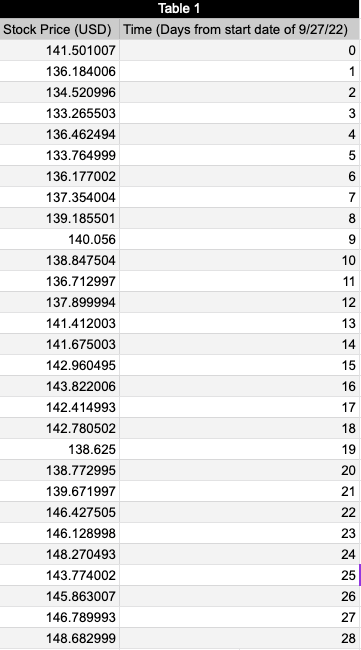
\includegraphics[width = 8cm]{Images/Table_1}\]
	Table 2 shows the differential approach to deriving the differential equation model. As the stochastic part cannot be derived, only the derivation of the deterministic part is shown. Columns 1 and 2 are simply copied from Table 1. Equations 1 and 2 are used to derive the changes in stock price \(S_t\) and time \(t\), put into columns 3 and 4 respectively. The derivative of \(S_t\) with respect to \(t\) can be approximated as \(\Delta S_t/\Delta t\), as shown in column 5. The stock price \(S_t\) is then listed again, as the plot is of \(\Delta S_t/\Delta t\) vs \(S_t\).
	\[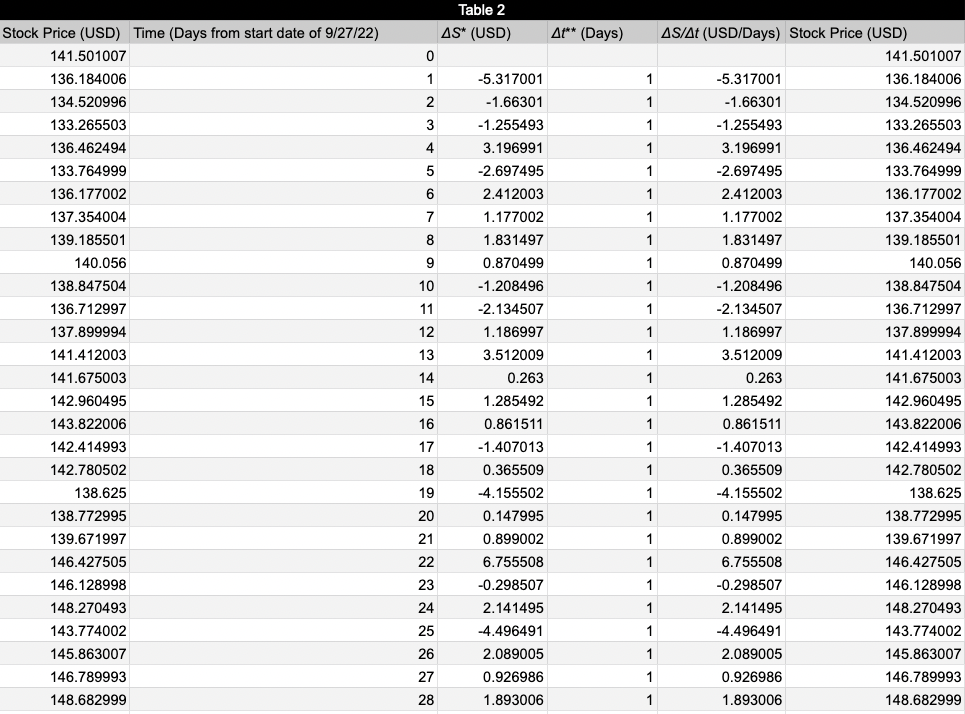
\includegraphics[width = 18cm]{Images/Table_2}\]
	\begin{align*}
		\Delta S_{t, i} &= S_{t, i} - S_{t, i - 1} \tag{Equation \(1^{*}\)} \\
		\Delta t_i &= t_i - t_{i - 1} \tag{Equation \(2^{**}\)}
	\end{align*}
	This is the graph of \(\Delta S/\Delta t\) (in USD/day) vs \(S\) (in USD) with a linear regression performed.
	\[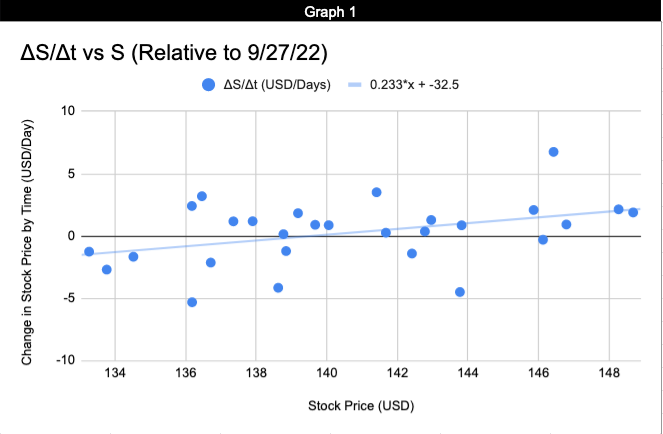
\includegraphics[width = 10cm]{Images/Graph_1}\]
	It is clear that there is a linear relationships between the stock price and its derivative with respect to time. It can therefore be said that
		\[\dv{S_t}{t} \propto S_t \implies \dv{S_t}{t} = \mu S_t\]
		where \(\mu\) is a constant. Using information from Stochastic Calculus: An Introduction with Applications \cite{Stochastic}, the Wiener process can be appended, adding the random motion to the model:
		\[\dv{S_t}{t} = \mu S_t + \sigma S_t\dv{W_t}{t}\]
		where \(S_t\) is stock price as a function of time \(t\), \(\mu\) is the (constant) drift, \(\sigma\) is the (constant) volatility, and \(W_t\) is a standard Wiener process. \\
		The Wiener process is stochastic, meaning that its value changes over time randomly. As such, only the distribution of possible values is known at any given point in time. This distribution is defined by the mean and variance, in this case 0 and 1 respectively. The Wiener process is a series of randomly distributed normal variables with variances that increase over time, reflecting the increasing uncertainty in making predictions further into the future. \\
		The dependent variable \(t\) is not present, making this an autonomous DE. The only information needed for the model are \(\mu\), \(\sigma\), and the initial stock price \(S_0\). \\
	\(\mu\) is the amount that \(\Exp(S_t)\), the expected value of the stock price, changes per year, making it the coefficient of the linear regression of \(\Delta S_t/\Delta t\) against \(S_t\) divided by 365, so \(\mu \approx 0.00064\).\\
	\(\sigma\) is simply the standard deviation of the stock price in the sample, so 
		\[\sigma = \sqrt{\frac{\sum\limits_{i = 1}^n(S_{t, i} - \bar{S}_{t})^2}{n - 1}} \approx 4.356\]
		where \(n\) is the number of days sampled, \(S_{t, 1 \cdots n}\) are the particular stock prices, and \(\bar{S}_t\) is the average stock price in the sample:
		\[\bar{S}_t = \frac{\sum\limits_{i = 1}^nS_{t,i}}{n}\]
	The model then becomes
		\[\boxed{\dv{S_t}{t} = 0.00064S_t + 4.356S_t\dv{W_t}{t}}\]
	\begin{thebibliography}{1}
		\bibitem{Yahoo}
			Yahoo Finance,
			\textit{Alphabet Inc. (GOOG) Stock Price, News, Quote \& history - Yahoo Finance},
			New York, NY,
			2022.
		\bibitem{Stochastic}
			Gregory F. Lawler,
			\textit{Stochastic Calculus: An Introduction with Applications},
			Chicago, IL, 
			2014.
	\end{thebibliography}
\end{document}
